\section{Análisis de las Trayectorias Óptimas}
Una vez identificados los ángulos de lanzamiento que minimizan la distancia de aproximación a Venus, se procede a analizar en detalle las trayectorias correspondientes a los dos puntos óptimos encontrados en las dos ventanas de interés.

\subsection{Primer Punto Óptimo (Ventana 1)}
Este punto, con ángulos de Guiñada $\varphi = -8.395^\circ$ y Cabeceo $\theta = -0.820^\circ$, corresponde a una maniobra que resulta en una \textbf{pérdida de energía} de la nave, cumpliendo el objetivo de acercarse al Sol.

\begin{figure}[H]
    \centering
    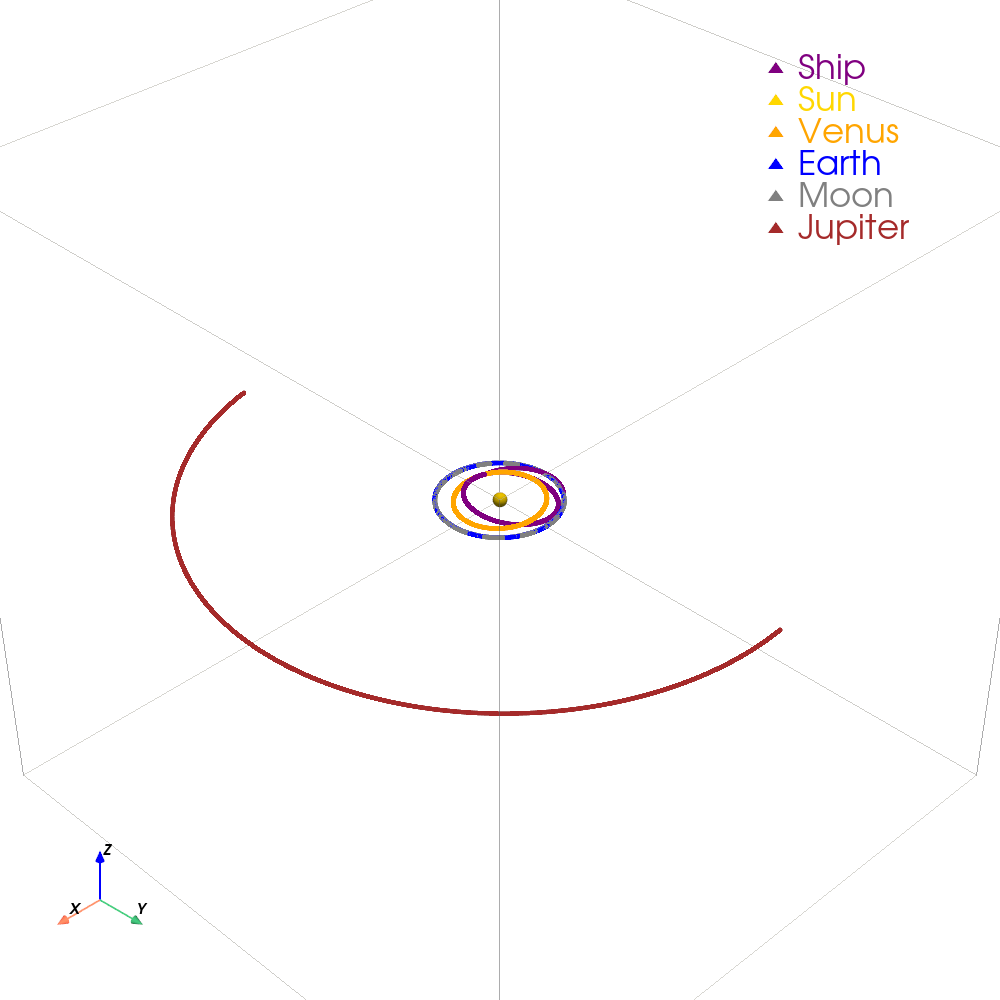
\includegraphics[width=0.8\textwidth]{graphs/acercamiento/orbit_plot_1.png}
    \caption{Trayectoria 3D de la simulación óptima (acercamiento).}
\end{figure}

\begin{figure}[H]
    \centering
    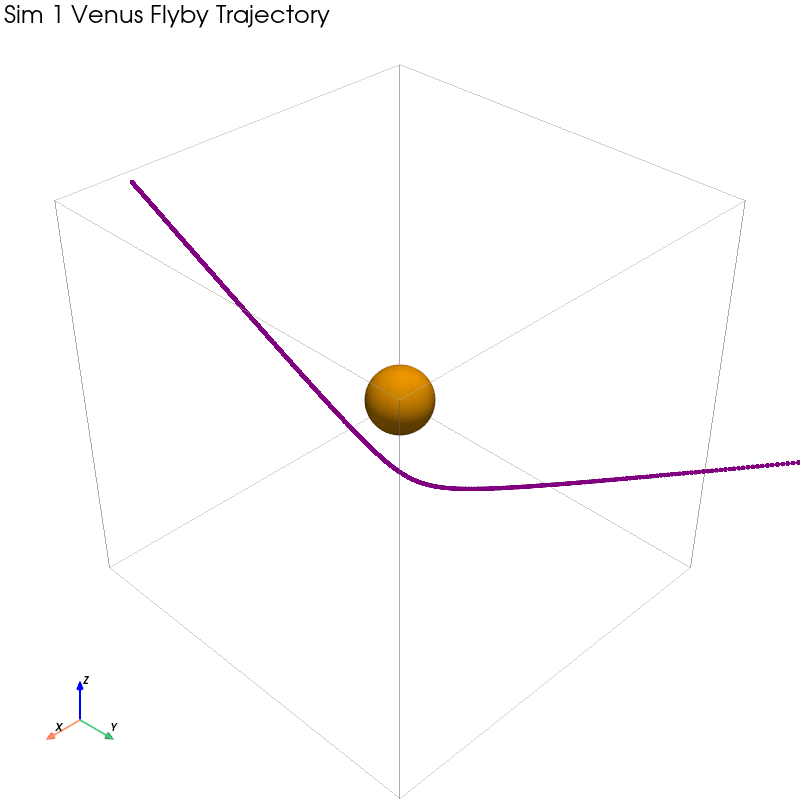
\includegraphics[width=0.5\textwidth]{graphs/acercamiento/venus_flyby_static_1.png}
    \caption{Detalle de la trayectoria hiperbólica durante el sobrevuelo de Venus (acercamiento).}
\end{figure}

\begin{figure}[H]
    \centering
    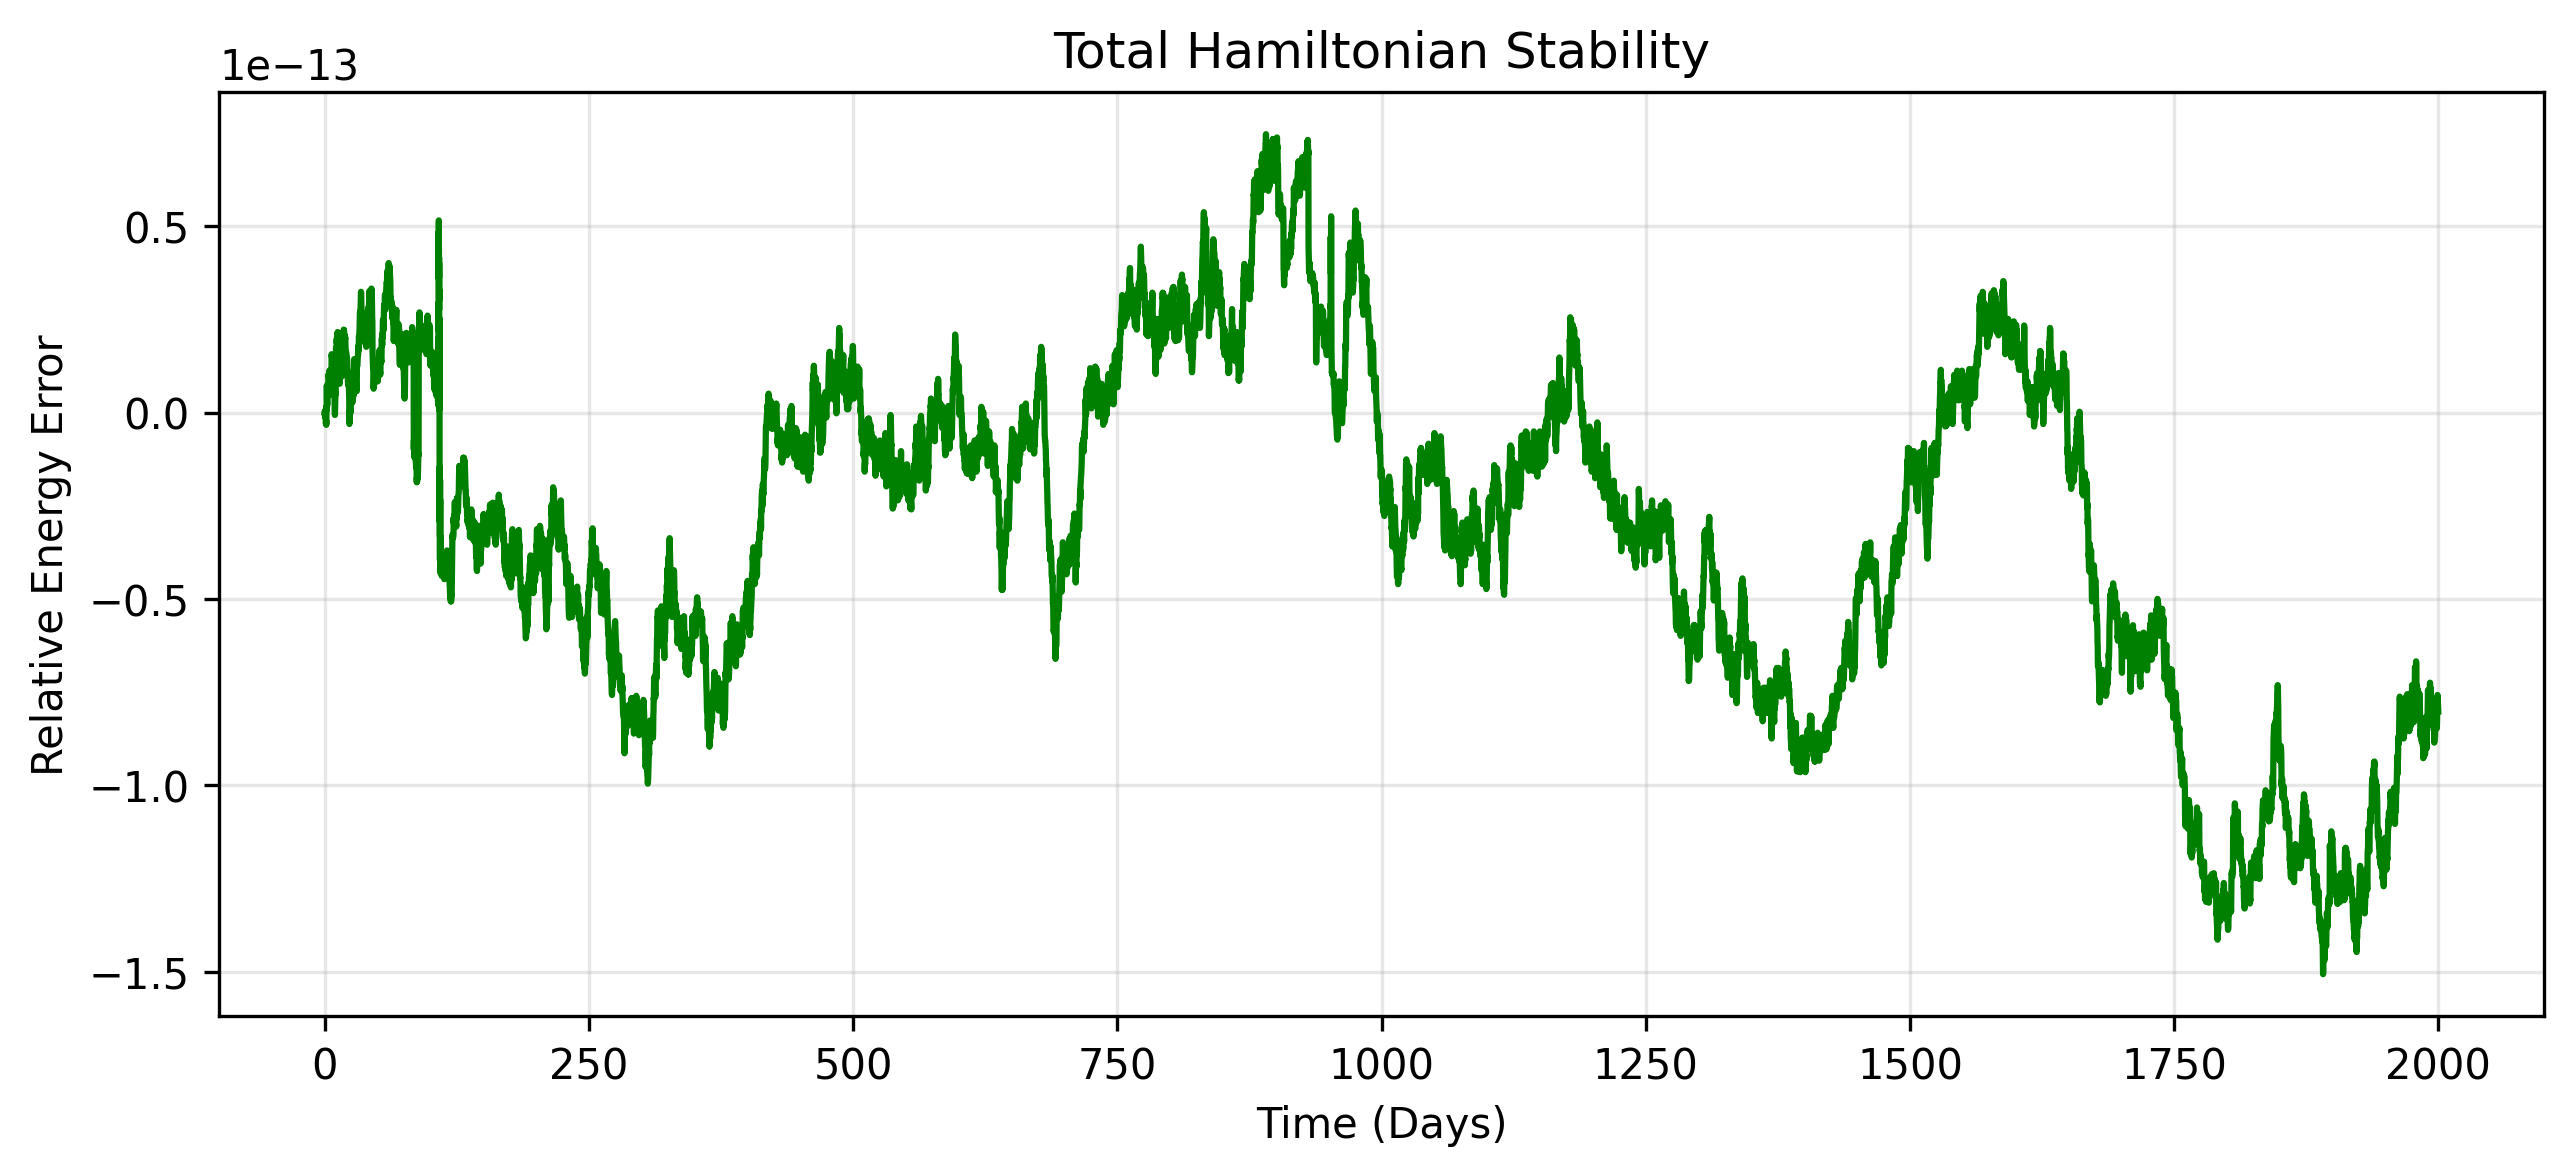
\includegraphics[width=0.8\textwidth]{graphs/acercamiento/total_energy_1.png}
    \caption{Error relativo de la energía total del sistema (acercamiento).}
\end{figure}

\begin{figure}[H]
    \centering
    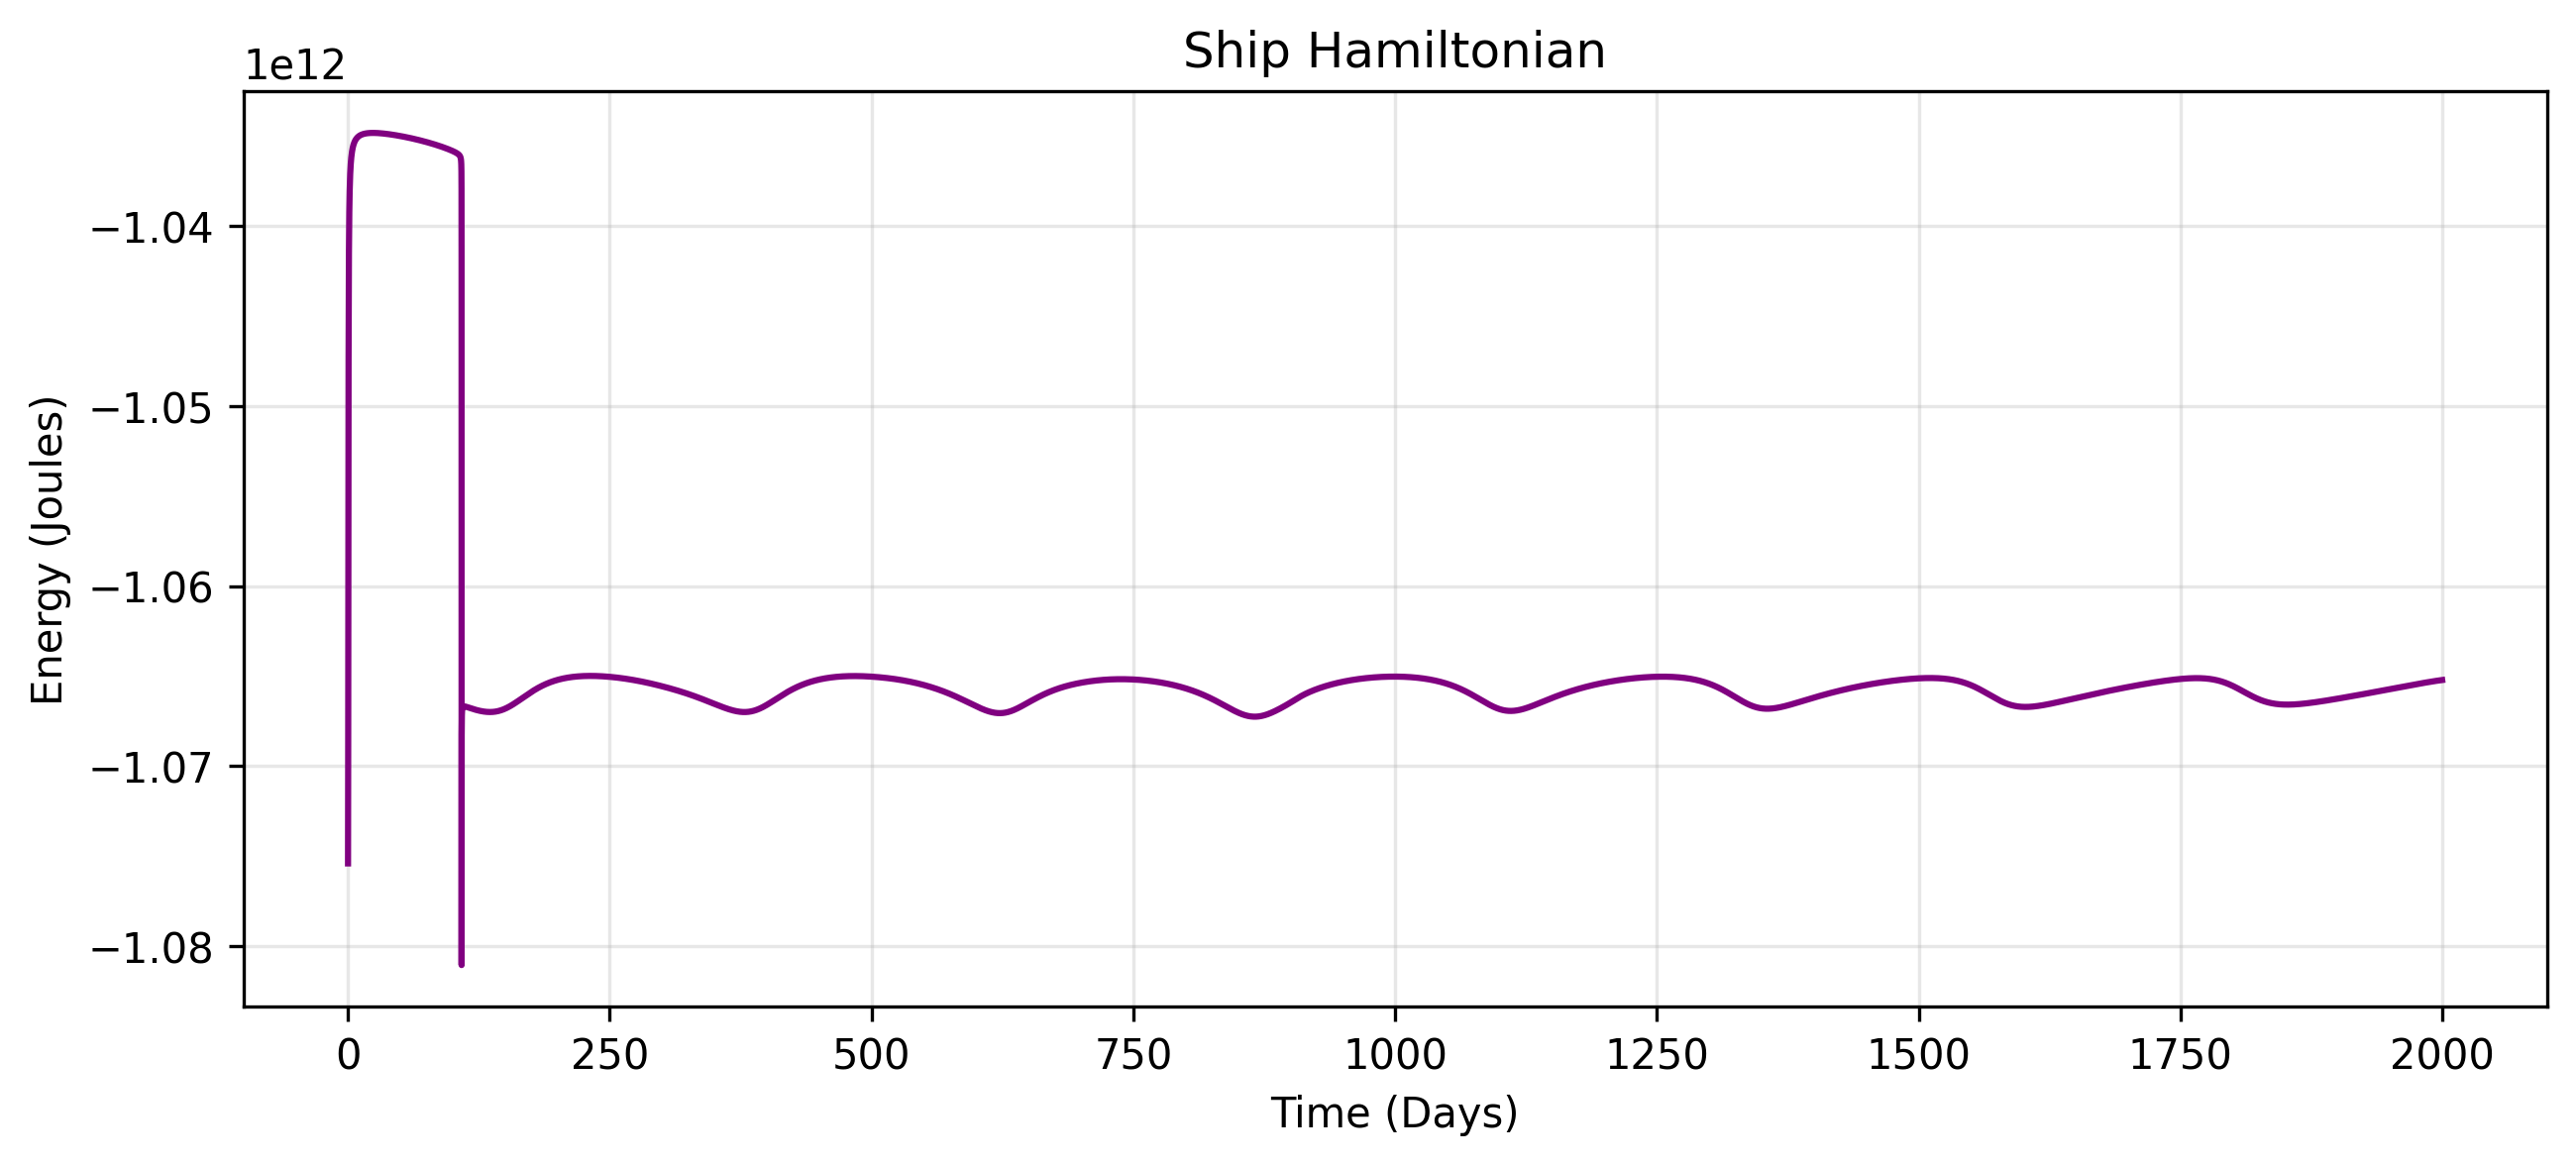
\includegraphics[width=0.8\textwidth]{graphs/acercamiento/ship_energy_1.png}
    \caption{Energía específica de la nave (acercamiento). Se observa un salto energético negativo ($\Delta E \approx -2.9 \cdot 10^{10}$ J) tras el encuentro con Venus, así como un pequeño bug al inicio.}
\end{figure}

\subsection{Segundo Punto Óptimo (Ventana 2)}
Este segundo punto, con ángulos de Guiñada $\varphi = 1.745^\circ$ y Cabeceo $\theta = -2.105^\circ$, corresponde a una maniobra que resulta en una \textbf{ganancia de energía} de la nave. Aunque no cumple el objetivo principal, es un resultado físicamente interesante.

\begin{figure}[H]
    \centering
    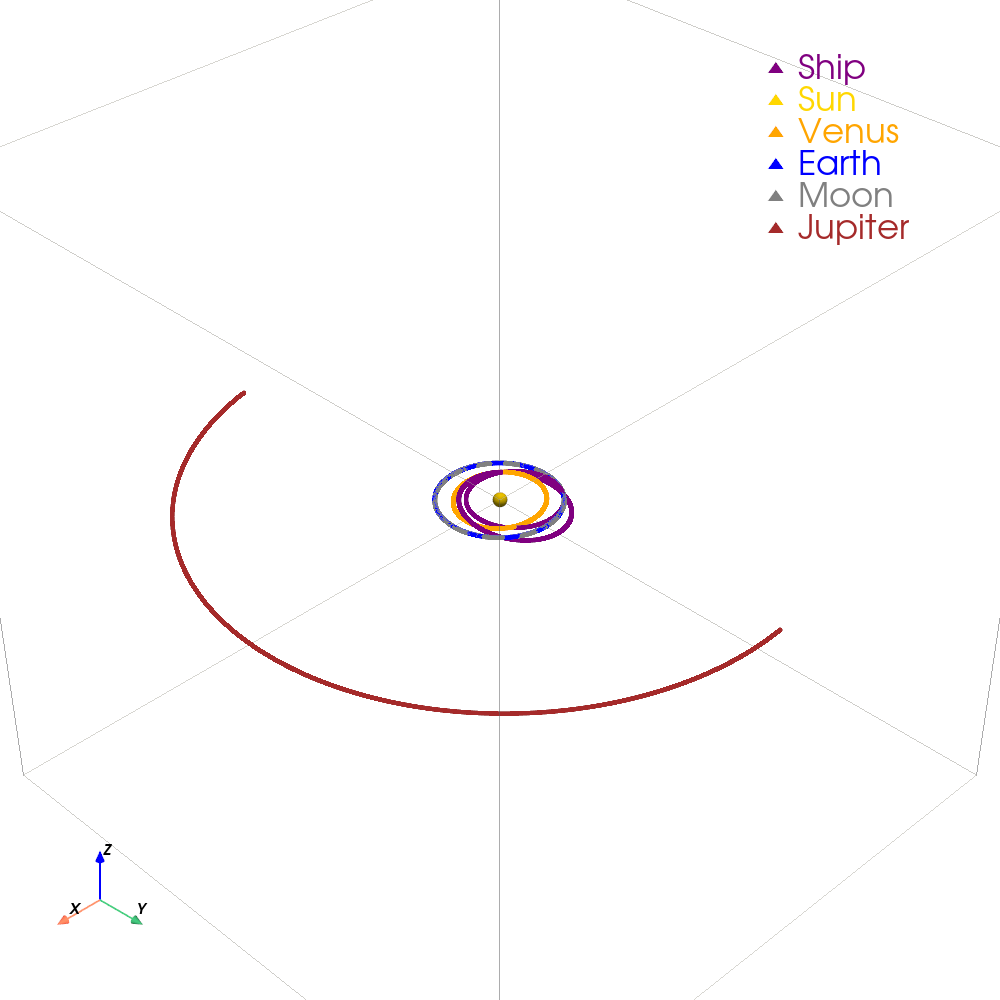
\includegraphics[width=0.8\textwidth]{graphs/alejamiento/orbit_plot_1.png}
    \caption{Trayectoria 3D de la simulación óptima (alejamiento).}
\end{figure}

\begin{figure}[H]
    \centering
    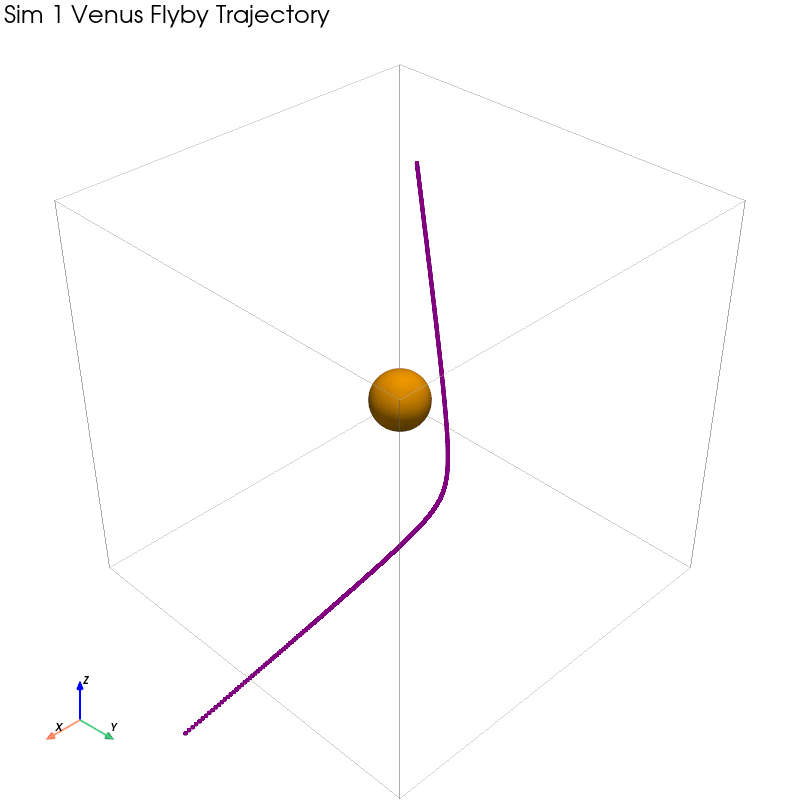
\includegraphics[width=0.5\textwidth]{graphs/alejamiento/venus_flyby_static_1.png}
    \caption{Detalle de la trayectoria hiperbólica durante el sobrevuelo de Venus (alejamiento).}
\end{figure}

\begin{figure}[H]
    \centering
    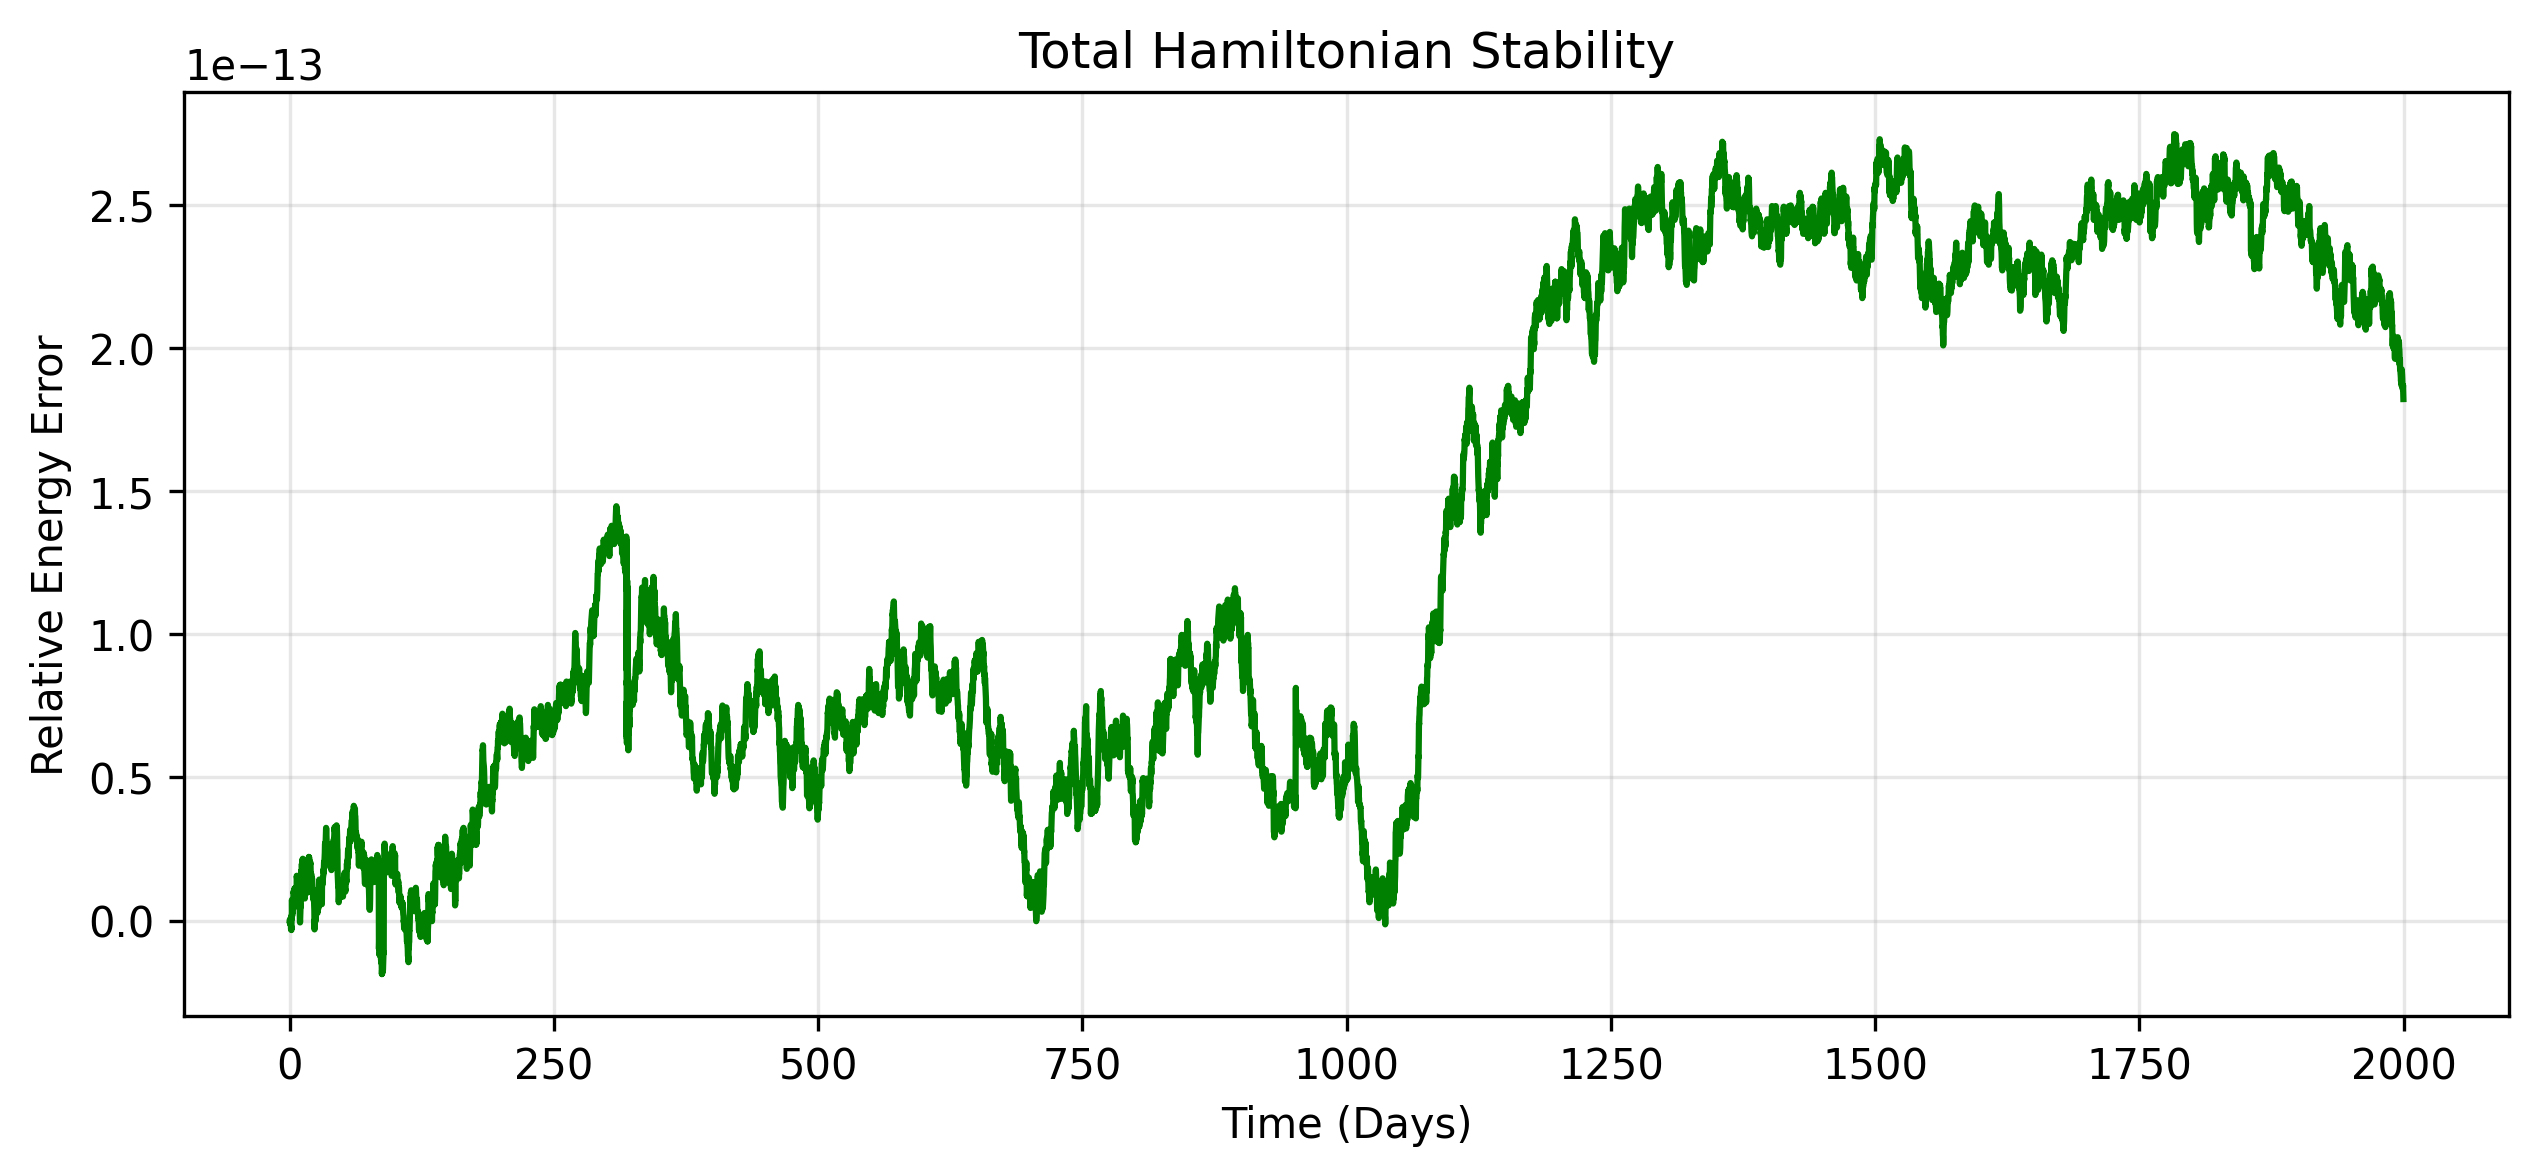
\includegraphics[width=0.8\textwidth]{graphs/alejamiento/total_energy_1.png}
    \caption{Error relativo de la energía total del sistema (alejamiento).}
\end{figure}

\begin{figure}[H]
    \centering
    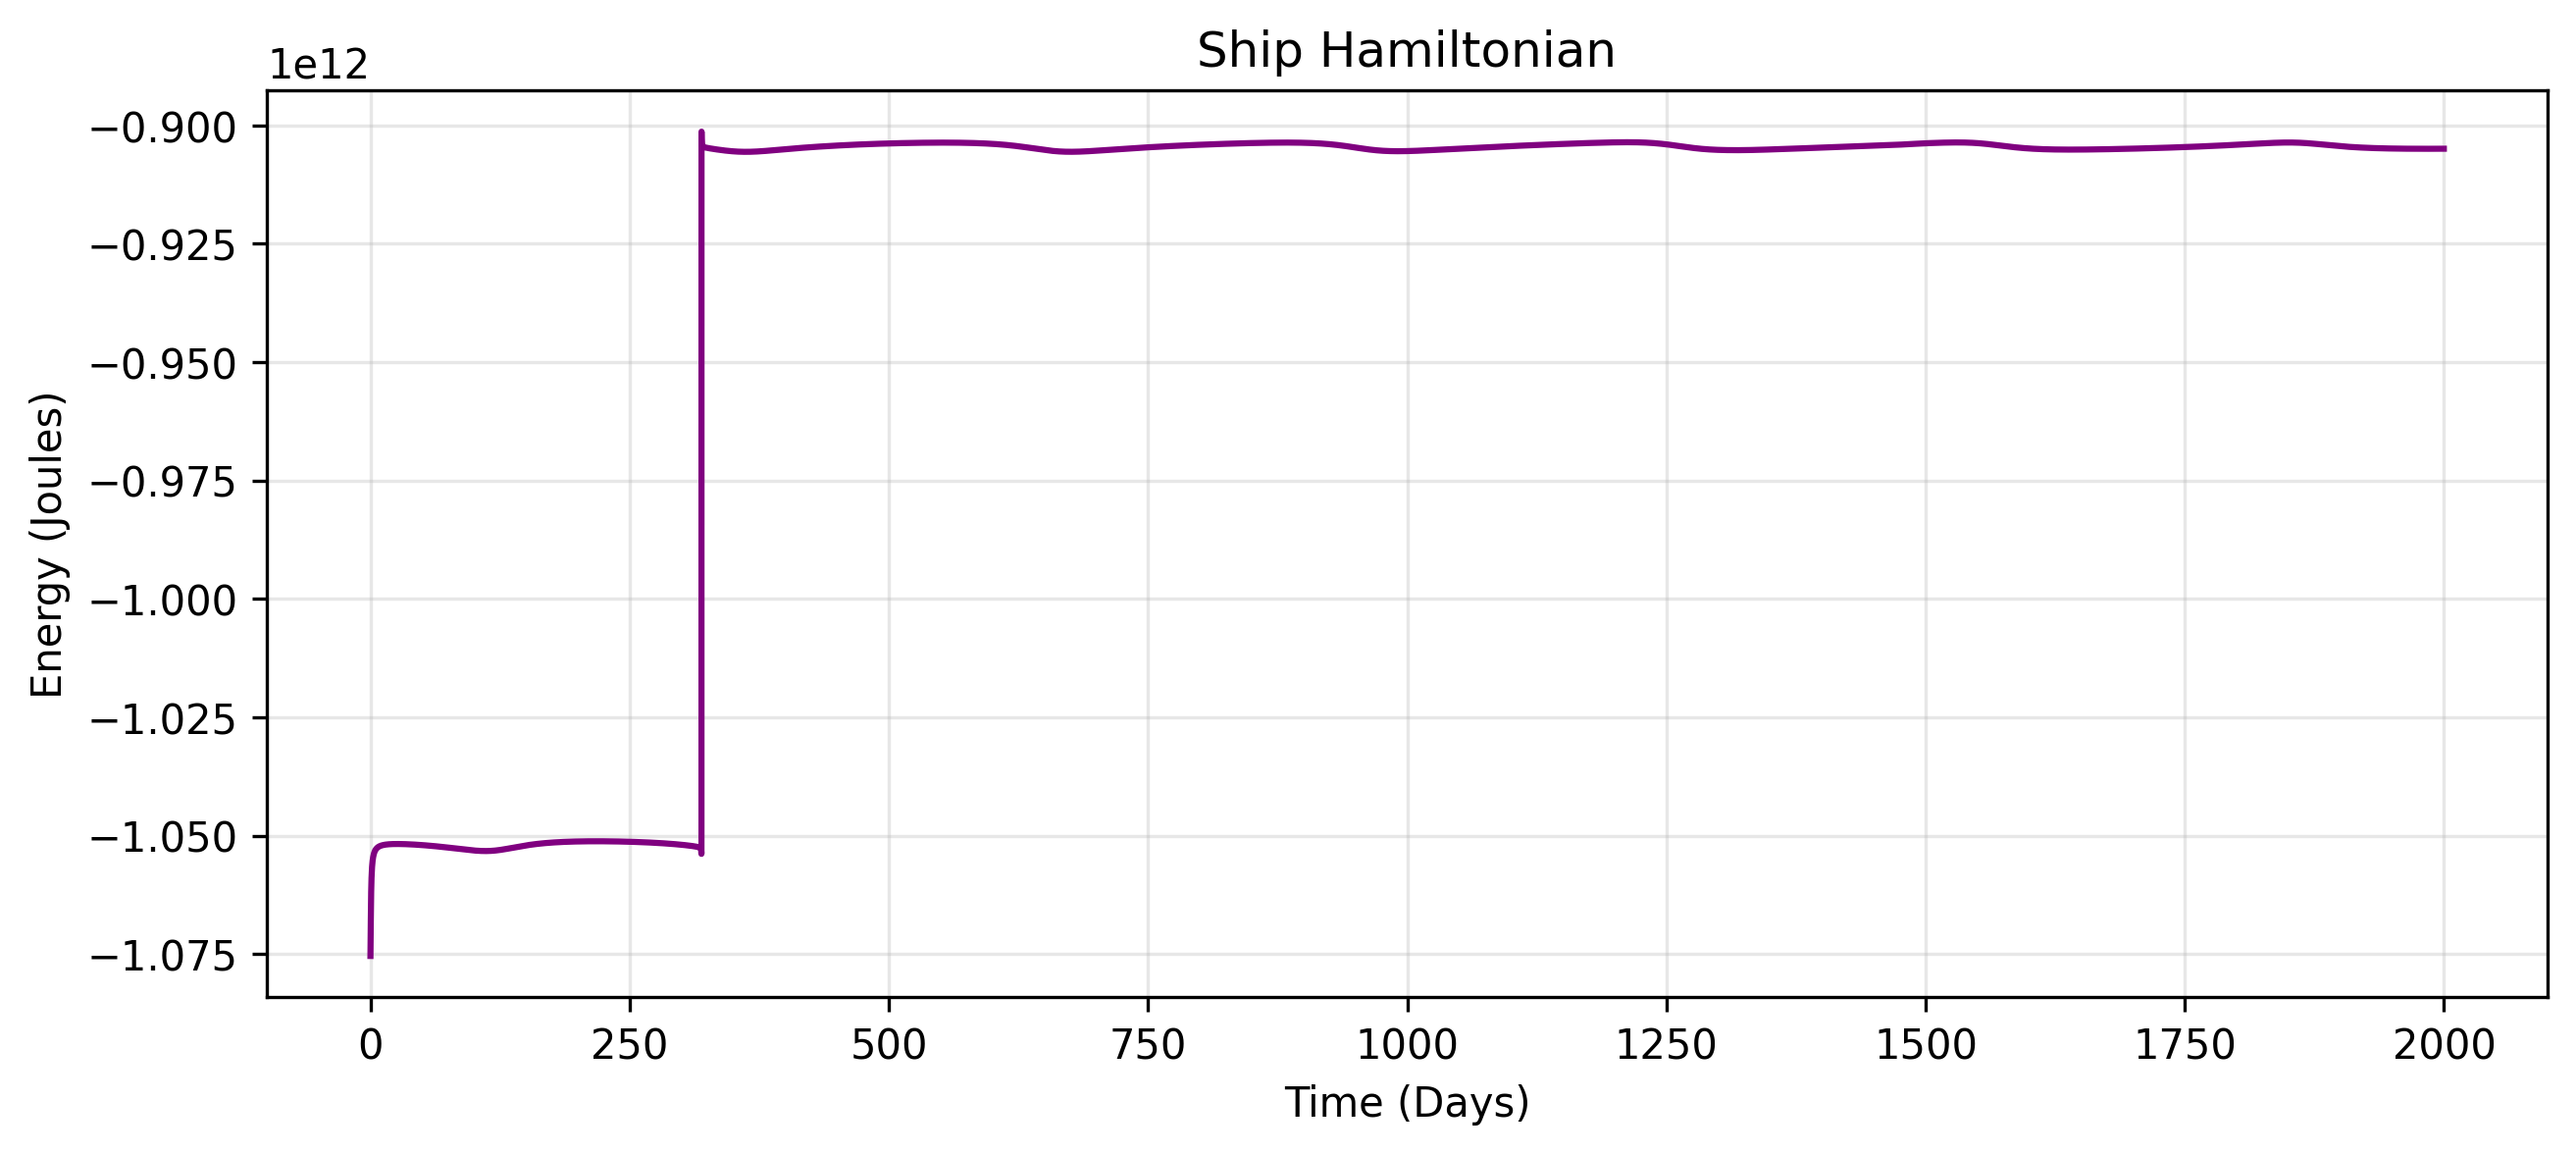
\includegraphics[width=0.8\textwidth]{graphs/alejamiento/ship_energy_1.png}
    \caption{Energía específica de la nave (alejamiento). Se observa un salto energético positivo ($\Delta E \approx +1.7 \cdot 10^{11}$ J) tras el encuentro con Venus.}
\end{figure}

\subsection{Vídeos y HTML Interactivo}
Adicionalmente, se han generado vídeos de la simulación completa y de la maniobra de aproximación a Venus, 
así como un \textit{html} interactivo de la órbita tridimensional en el Sistema Solar, que se pueden 
encontrar tanto en la carpeta de resultados adjunta como en el GitHub.